\documentclass[11pt]{beamer}
\usepackage[utf8]{inputenc}
\usepackage[T1]{fontenc}
%\usepackage{natbib}
\usetheme{Pittsburgh}
\usepackage{verbatim} 
\usepackage[english]{babel}
\usepackage{epstopdf}
%\titlegraphic{%\vspace*{1cm}
%	\includegraphics[width=2.5cm]{logo_udelar}
	%\hspace*{1cm}~%
%		\includegraphics[width=3.5cm]{logo_FCEA.png}
%}
\setbeamertemplate{navigation symbols}{}
\setbeamertemplate{footline}[frame number]
\AtBeginSection{ 
	\begin{frame}
		\frametitle{Index}
			\tableofcontents[currentsection]
	\end{frame}
}
\begin{document}
	\title{Modelos dinámicos y computacionales en Economía}
	\subtitle{Introducción a NetLogo}
	%\logo{}
	\institute{Licenciatura en Economía, FCEA, UDELAR}
	\date{17 de octubre de 2023}

	
	%\subject{}
	%\setbeamercovered{transparent}
	%\setbeamertemplate{navigation symbols}{}
	\frame[plain]{
	\begin{figure}
	\centering
	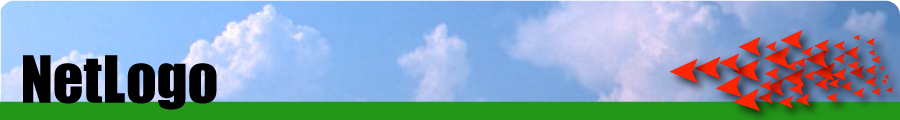
\includegraphics[width=0.7\linewidth]{figuras/netlogo-title-wide-60.jpg}
	%		\caption{}
	\label{fig:netlogo-title-wide-60}
\end{figure}	
		\vspace{-1cm}
\maketitle
}
%\setbeamertemplate{background}{\includegraphics[width=2 cm]{logo_FCEA.png}}

\begin{frame}
\frametitle{Contenido de la clase:}
\begin{itemize}
	\item Presentación de Netlogo
	\item Principios del diseño
	\item Interfaz
	\item Clases / objetos en NetLogo
	\item Ejemplo: Pila de arena
	\item Ejemplo: Fire model	
\end{itemize}
\end{frame}

\begin{frame}
	\frametitle{Modelos}
\begin{itemize}
\item ¿qué es un modelo?\\
``...Since all models are wrong the scientist cannot obtain a "correct" one by excessive elaboration. On the contrary following William of Occam he should seek an economical description of natural phenomena. Just as the ability to devise simple but evocative models is the signature of the great scientist so overelaboration and overparameterization is often the mark of mediocrity.
\\Since all models are wrong the scientist must be alert to what is  importantly wrong. It is inappropriate to be concerned about mice when there are tigers abroad''.\footnote{Box, G. E. (1976). Science and statistics. \textit{Journal of the American Statistical Association, 71}(356), 791-799.}

\item ¿qué es un modelo basado en agentes?
\item ¿qué es un agente?
\end{itemize}

\end{frame}

\begin{frame}
\frametitle{Presentación de NetLogo}
\begin{itemize}
%	\item is a premier agent-based modeling language and development environment,	designed by Uri Wilensky at Northwestern University.
%	It is the most widely used ABM environment.
%	It’s the easiest to learn.
	\item Es un lenguaje de programación y un entorno de desarrollo (IDE), diseñado por Uri Wilensky de Northwestern University.
	\item Es uno de los entornos de programación más utilizados para Modelos Basados en Agentes (ABM).
	\item Es el más fácil de aprender.
	\item Especialmente diseñado para estudiar la dinámica de sistemas complejos.
\end{itemize}
\end{frame}

\begin{frame}
\frametitle{Principios del diseño}
\begin{itemize}
	\item Bajo coste de aprendizaje
	\begin{itemize}
		\item Pueden construirse modelos simples en poco tiempo
		\item Interfaz gráfica intuitiva
		\item Programación Orientada a Objetos
	\end{itemize}
	\item Alta performance
	\begin{itemize}
		\item El lenguaje permite modelos a gran escala. 
		\item Permite leer, modificar y publicar modelos.
		\item Elimina las diferencias entre el investigador y el programador.
		\item Permite desarrollo e investigación interactivas.
		\item Permite compartir modelos.
	\end{itemize}
\end{itemize}
\end{frame}

\begin{frame}
\frametitle{¿Qué tan "complicado" puede llegar a ser?}
\begin{itemize}
	\item Decenas de miles de "agentes", "zonas" y "links".
	\item Decisiones complejas
	\item Muchos tipos de agentes
	\item Modelos de ciudades enteras
	\item Herramientas adicionales (extensiones) permiten la integración con otros software.
	\item Tipos de análisis
	\begin{itemize}
		\item Modelos espaciales
		\item Análisis de políticas
		\item Propagación de información (marketing, redes)
		\item Sistemas de apoyo en la toma de decisiones
	\end{itemize}
\end{itemize}
\end{frame}

\begin{frame}
	\frametitle{¿Qué tan "complicado" puede llegar a ser?}
	\framesubtitle{Ejemplo: Esquema de interacciones en un ABM macroeconómico.}
% TODO: \usepackage{graphicx} required
\begin{figure}
	\centering
	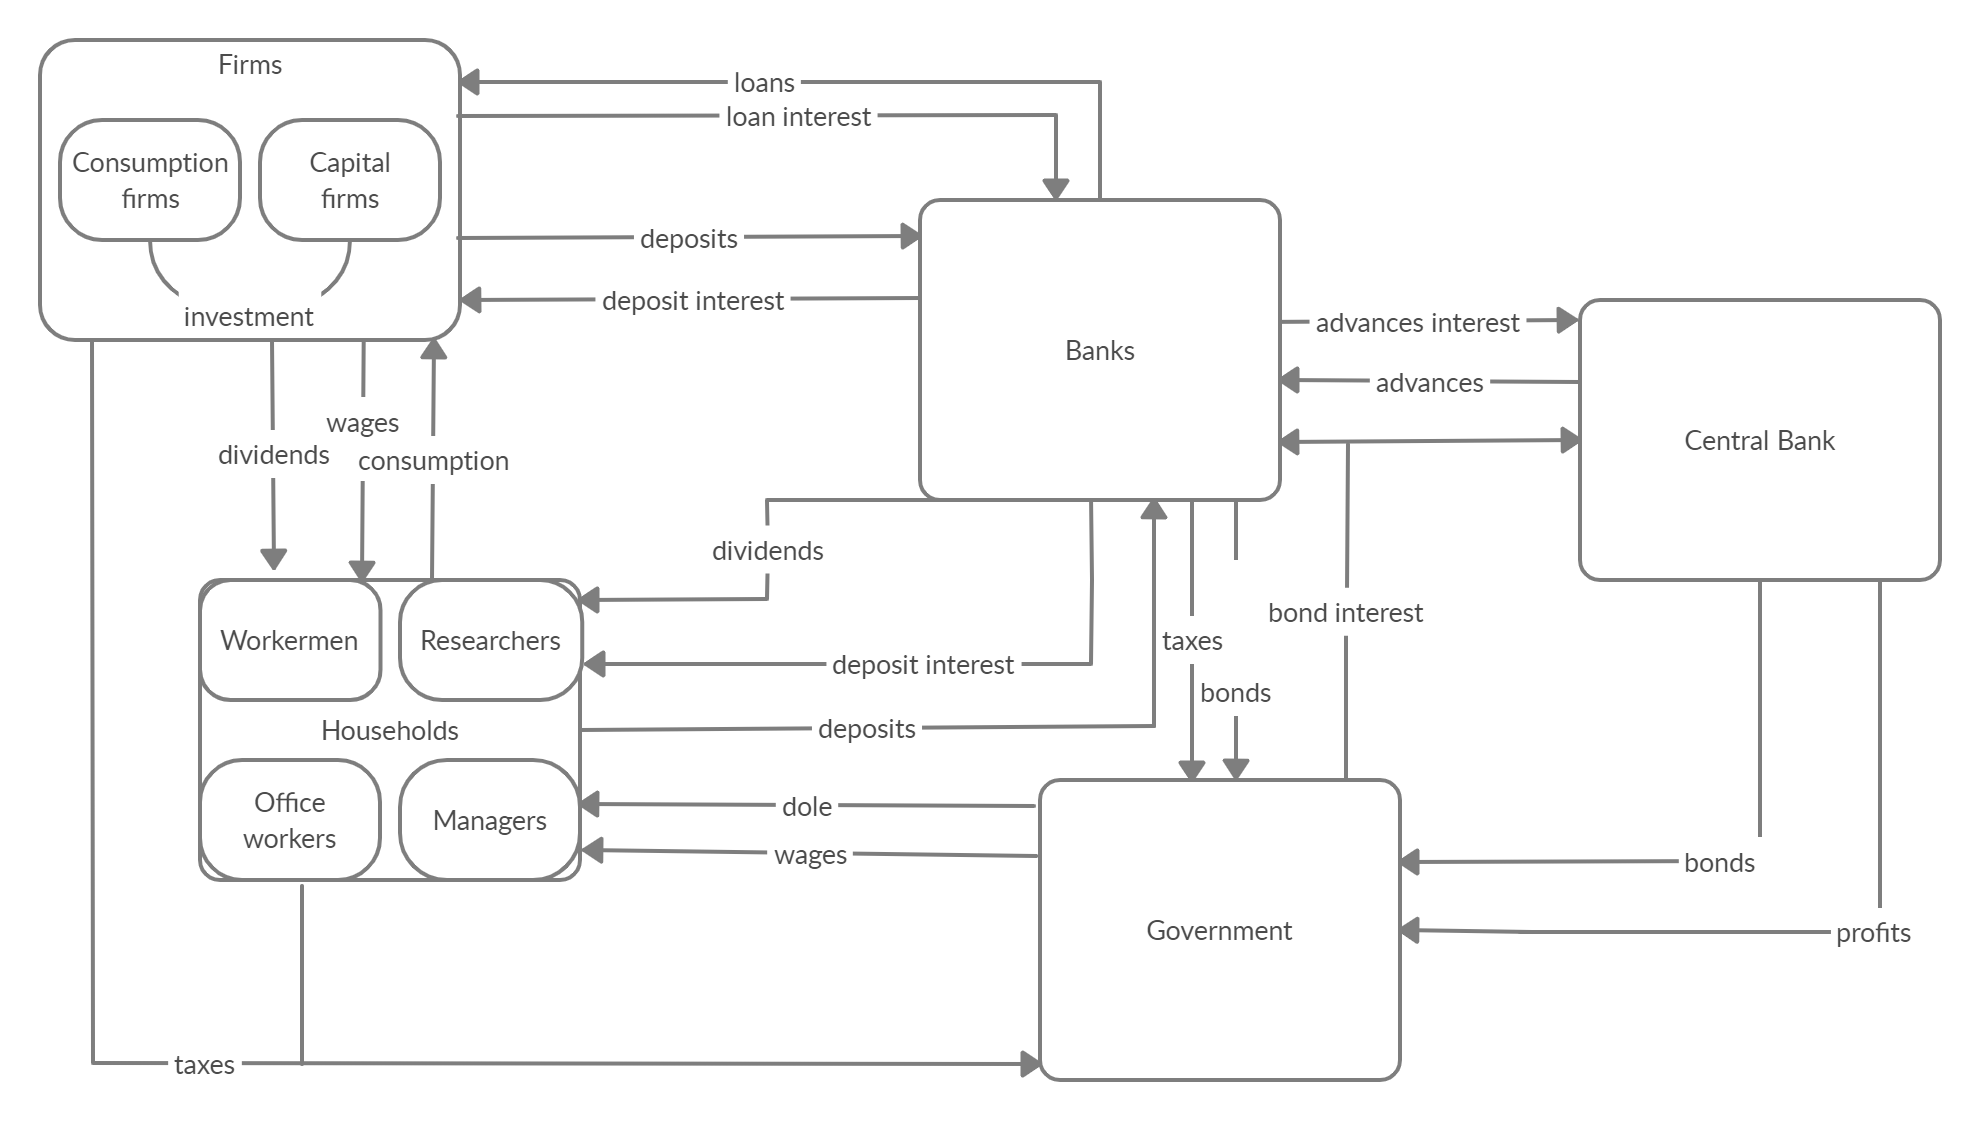
\includegraphics[width=0.9\linewidth]{figuras/diagram.jpg}
%	\caption{Esquema de interacciones en un ABM macroeconómico.}
	\label{fig:diagram}
\end{figure}

\end{frame}


\begin{frame}
\frametitle{¿Cómo podemos utilizar el análisis de sistemas complejos?}
\begin{itemize}
	\item Los sistemas complejos pueden ser muy difíciles de predecir, controlar y manejar.
	\item Sin embargo, en muchos casos el objetivo de las políticas públicas consiste precisamente en procurar predecir, controlar y manejar estos sistemas.
	\item El análisis de sistemas complejos y los modelos basados en agentes nos permiten usar un "simulador de vuelo" más que una predicción certera.
\end{itemize}
\end{frame}

\begin{frame}
\frametitle{Aspectos a tomar en cuenta:}
\begin{itemize}
	\item Tipping points: puntos donde el sistema puede cambiar de régimen -fase- a partir de un pequeño cambio en los parámetros.
	\item Irreversibilidad: las posibilidades futuras se encuentran determinadas por elecciones pasadas.
	\item Alta sensibilidad a las condiciones iniciales: "el presente determina el futuro, pero una aproximación del presente no determina aproximadamente el futuro" (Lorenz).
	\item No linealidad: los insumos no afectan a los resultados de forma lineal.
	\item Individuos diversos y heterogéneos.
	\item Los individuos se encuentran interconectados y afectan a las decisiones de los demás.
\end{itemize}
\end{frame}

\begin{frame}
\frametitle{Una tercera forma de hacer ciencia}
\framesubtitle{Axelrod (1997)}
\begin{itemize}
	\item Dos formas tradicionales de hacer ciencia: 
	\begin{itemize}
		\item Inducción: desde lo particular a una teoría general
		\item Deducción: desde los principios fundamentales a una teoría.
	\end{itemize}
	\item Una tercera forma:
	\begin{itemize}
		\item "Generativa". Utiliza principios fundamentales para generar un set de datos que permita avanzar hacia una teoría general.
	\end{itemize}
\end{itemize}
\end{frame}

\begin{frame}
\frametitle{Bottom-up / Up-bottom}
\begin{itemize}
	\item Si conocemos las reglas de comportamiento individuales, ¿podemos determinar el patrón agregado?
	\begin{itemize}
		\item Este tipo de modelización nos permite un método para hacerlo.
	\end{itemize}
  	\item ¿Si conocemos el patrón agregado y queremos conocer las reglas de comportamiento individual? 
 	\begin{itemize}
 		\item Podemos proponer reglas y ver si generan el fenómeno agregado observado.
 	\end{itemize}
\end{itemize}
\end{frame}

\begin{frame}
\frametitle{NetLogo}
\begin{itemize}
	\item Tutoriales:
	\begin{itemize}
		\item En el sitio Web
		\item En \textbf{Ayuda / Guía del Usuario Netlogo}
		\item En \textbf{Ayuda / Diccionario Netlogo}
		\item En \textbf{Ayuda / Comunidad de Usuarios de Netlogo}
	\end{itemize}
	\item En la pantalla principal vemos tres pestañas:
	\begin{itemize}
		\item Ejecutar (interfaz)
		\item Información
		\item Código
	\end{itemize}
\item Al abrir un modelo, en la interfaz veremos siempre\footnote{Ver ejemplo de \textbf{Archivo / Biblioteca de Modelos / IABM Textbook / chapter 8 / "Run example"}}:
\begin{itemize}
	\item Botón "SETUP"
	\item Botón "GO"
	\item Selector de velocidad
	\item Opción de añadir otros elementos para la interfaz
\end{itemize}
\end{itemize}
\end{frame}

\begin{frame}
\frametitle{Algunos comandos para los agentes "turtles"}
\begin{itemize}
\small	\item create-turtles (crt): \textbf{create-turtles 100} 
	\item ask: ask turtles [set color blue set shape "car"]
	\item ask turtles [setxy random-xcor random-ycor]
	\item ask: ask patches [set pcolor white]
	\item forward (fd), backward (bk)
%	\item left (lt), right (rt)
	\item repeat
	\item color, size, xcor, ycor
	\item pen-down (pd), pen-up (pu)
	\item clear-all (ca)
	\item inspect / watch
	\item die
\end{itemize}
Importante: los comandos los podemos ingresar desde la línea de comandos o en la pestaña "Código".
\end{frame}

\begin{frame}
\frametitle{Zonas "patches"}
\begin{itemize}
	\item Podemos usar la opción "Inspect" (botón derecho del mouse o \textbf{inspect patch 0 0} )
	\item Cambiamos el color con \textbf{pcolor}:\\
	 \textbf{ask patch 0 0 [set pcolor blue]} \\
	 \textbf{ask patches [set pcolor green]}
	\item  Turtles pueden acceder directamente a la info de los patches.
	\item Comandos: 
	\begin{itemize}
		\item setxy, facexy
		\item random-xcor (pxcor), random-ycor (pycor)
	\end{itemize}
\end{itemize}
\end{frame}

\begin{frame}
\frametitle{Ejemplo: Pila de arena}
{\small ``Who could ever calculate the path of a molecule?
How do we know that the creations of worlds are not determined by falling grains of sand?'' \\ \textit{ -- Victor Hugo, Les Miserables}}
\vspace{0.6cm}\\
Los fenómenos complejos que se observan, indican que la naturaleza se encuentra en un estado críticamente auto-organizado\footnote{Bak, P., Tang, C., \& Wiesenfeld, K. (1987). Self-organized criticality: An explanation of the 1/f noise. \textit{Physical Review Letters, 59}(4), 381.}.
\vspace{0.6cm}\\

En \textbf{Archivo / Biblioteca de Modelos / IABM Textbook / chapter 8 / "Sandpile simple"}
\begin{itemize}
	\item ¿Cómo se distribuyen las avalanchas?
	\item ¿cuál es el estado crítico relevante en este modelo?
\end{itemize}
\end{frame}

\begin{frame}
\frametitle{Ejemplo: Fire model}
En \textbf{Archivo / Biblioteca de Modelos / IABM Textbook / chapter 3 / Fire extensions / "Fire simple"}
\begin{itemize}
	\item ¿Cuáles son los parámetros relevantes?
	\item ¿A partir de qué valores cambia el comportamiento del modelo?
	\item ¿Cómo cambia este modelo si modificamos el criterio por el cual se prende fuego un árbol?
	\begin{enumerate}
		\item Que observe a los ocho vecinos a su alrededor.
		\item Que los ``contagie'' con una probabilidad del 70\%.
	\end{enumerate}
	\item ¿Cómo podemos medirlo?
\end{itemize}
\end{frame}

\begin{frame}
	\frametitle{Ejemplo: Fire model (cont.)}
	\framesubtitle{BehaviorSpace}
	\begin{itemize}
		\item Cada vez que encontremos un modelo con componentes estocásticos, debemos correr varias veces el modelo para poder caracterizarlo.
		\begin{itemize}
			\item Para encontrar su comportamiento ``promedio''.
			\item Para encontrar si existe un comportamiento anómalo o errático que es inherente al modelo.
		\end{itemize}
	\item NetLogo tiene disponible la herramienta BehaviorSpace, que permite correr un modelo repetidas veces.
	\item Con los mismos valores de los parámetros o con distintos valores. 
	\end{itemize}
\end{frame}

\begin{frame}
	\frametitle{Ejemplo: Fire model (cont.)}
	\framesubtitle{BehaviorSpace}
\underline{Experimento 1}
	\begin{itemize}
		\item Analizamos la cantidad de árboles quemados, para una densidad entre 40\% y 80\%. 
	\end{itemize}
\underline{Experimento 2}
\begin{itemize}
	\item Analizamos la cantidad de árboles quemados, considerando:
	\begin{itemize}
		\item una densidad entre 50\% y 80\%. 
		\item Una probabilidad de propagación entre el 65\% y el 100\%. 
	\end{itemize}
\end{itemize}
\end{frame}
\end{document}